% --------------------------------------------------------------
% This is all preamble stuff that you don't have to worry about.
% Head down to where it says "Start here"
% --------------------------------------------------------------
 
\documentclass[12pt]{article}
 
\usepackage[margin=1in]{geometry} 
\usepackage{amsmath,amsthm,amssymb}

\usepackage[thmmarks, amsmath, thref]{ntheorem}
\usepackage{enumerate}
\usepackage{multicol}
\usepackage{tikz}
\usepackage{xcolor}

 
\newcommand{\N}{\mathbb{N}}
\newcommand{\Z}{\mathbb{Z}}
 
\newenvironment{theorem}[2][Theorem]{\begin{trivlist}
\item[\hskip \labelsep {\bfseries #1}\hskip \labelsep {\bfseries #2.}]}{\end{trivlist}}
\newenvironment{lemma}[2][Lemma]{\begin{trivlist}
\item[\hskip \labelsep {\bfseries #1}\hskip \labelsep {\bfseries #2.}]}{\end{trivlist}}
\newenvironment{exercise}[2][Exercise]{\begin{trivlist}
\item[\hskip \labelsep {\bfseries #1}\hskip \labelsep {\bfseries #2.}]}{\end{trivlist}}
\newenvironment{problem}[2][Problem]{\begin{trivlist}
\item[\hskip \labelsep {\bfseries #1}\hskip \labelsep {\bfseries #2.}]}{\end{trivlist}}
\newenvironment{question}[2][Question]{\begin{trivlist}
\item[\hskip \labelsep {\bfseries #1}\hskip \labelsep {\bfseries #2.}]}{\end{trivlist}}
\newenvironment{corollary}[2][Corollary]{\begin{trivlist}
\item[\hskip \labelsep {\bfseries #1}\hskip \labelsep {\bfseries #2.}]}{\end{trivlist}}

\theoremstyle{nonumberplain}
\theoremheaderfont{\itshape}
\theorembodyfont{\upshape}
\theoremseparator{.}
\theoremsymbol{\ensuremath{\square}}
\newtheorem{proof}{Proof}
\theoremsymbol{\ensuremath{\square}}
\newtheorem{solution}{Solution}
\theoremseparator{. ---}
\theoremsymbol{\mbox{\texttt{;o)}}}
\newtheorem{varsol}{Solution (variant)}

% code listing settings
\usepackage{listings}
\lstset{
    language=Python,
    basicstyle=\ttfamily\small,
    aboveskip={1.0\baselineskip},
    belowskip={1.0\baselineskip},
    columns=fixed,
    extendedchars=true,
    breaklines=true,
    tabsize=4,
    prebreak=\raisebox{0ex}[0ex][0ex]{\ensuremath{\hookleftarrow}},
    frame=lines,
    showtabs=false,
    showspaces=false,
    showstringspaces=false,
    numbers=left,
    numberstyle=\small,
    stepnumber=1,
    numbersep=10pt,
    captionpos=t,
    escapeinside={\%*}{*)}
}
 
\begin{document}
 
% --------------------------------------------------------------
%                         Start here
% --------------------------------------------------------------
 
\title{Problem 1 Write-up}%replace X with the appropriate number
\author{Trust the Stochastic Process\\
        (Eli Katz, Avi Mahajan, James Stroud)}
 
\maketitle

\section{Exact Calculation}
 In order to calculate the exact probability of the Warriors not losing consecutive games for an 82 game season if they had a 80\% chance of winning each game, we did the following:

We divided the season up into 81 two-game ``windows''. So Window 1 is
games 1 and 2; Window 2 is games 2 and 3. Then for each window, we calculated the probability of NOT losing both games in a window GIVEN the Warriors had not lost both games in any of the previous windows. For that calculation, there are two scenarios to consider:
\begin{itemize}
\item The Warriors had \textbf{won} the 2nd game of the previous window (which is, by definition, the first game of the current window)
\item The Warriors had \textbf{lost} the 2nd game of the previous window (which is, by definition, the first game of the current window)
\end{itemize}
We wrote a MATLAB script that calculated, for each window, the probability of not losing 2 games in the same 2-game window given that the Warriors had not previously lost consecutive games. Then to calculate the odds of the Warriors never losing consecutive games over the entire season, we simply multiplied the conditional probabilities for each window and got an answer of approximately 5.88\%.

To figure out what win percentage would the Warriors need to raise that probability to 50\%, I ran the same calculations but with all possible winning percentages from 80\% to 100\% and saw which one yielded a 50\% probability.


\section{Simulation}
Another method we used (to verify our probability) was a simulation in Python. The simulation generated a sample 82-game season (based on a winning percentage of 80\%), and simply calcuated the number of times where there were 2 consecutive losses. Based on 1 million simulations, we found that the average number of consecutive losses was 3.24 per season, with a standard deviation of 2.03. We also found that about 5.87\% of the total simulated seasons had 0 consecutive losses, which seems to agree with the exact probability above. Below is a histogram of the number of consecutive losses.

\begin{figure}
  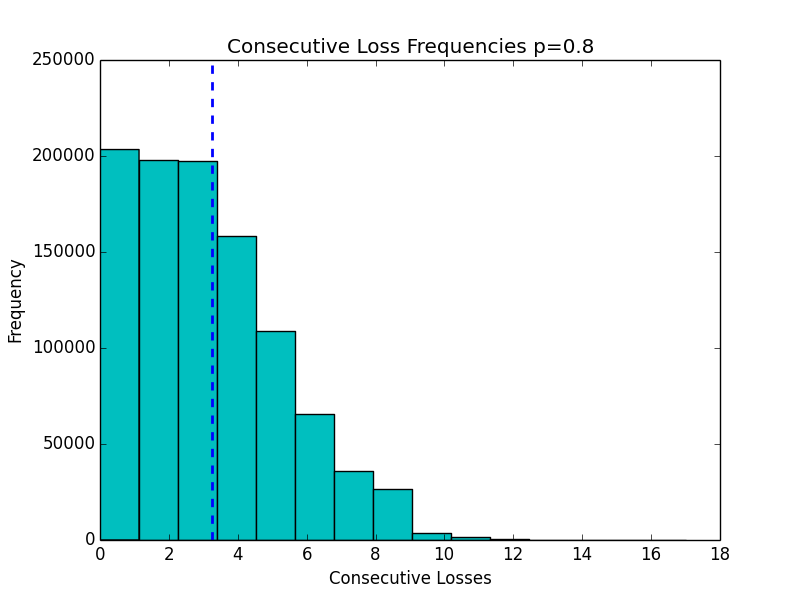
\includegraphics[width=\linewidth]{figure_1.png}
  \caption{Histogram of the results of the simulation. The average is marked by the dark blue line}
  \label{fig:boat1}
\end{figure}


\section{Part b: Testing the Hypothesis}
(see \lstinline|sample_out.txt| for sample outputs)

Let's assume that the null hypothesis is $H_0: \mu = 0$, and the one-sided alternative hypothesis is $H_A: \mu > 0$, where $\mu$ is the average number of consecutive losses in a season, over \textit{every} season, assuming the Warriors have a 80\% chance of winning. Using our simulation code, we can generate a sample of $n=$ 1 million simulated seasons and count the number of pairs of consecutive-losses in each. Through our simulation code, we find that the average number of consecutive losses per season in the sample is 3.2244, and the sample standard deviation is 2.0425. 

Through our stats program, we find that the p-value is less than 0.00001 (it's actually less than $1\times 10^{-8}$, but 0.00001 is the ``accepted" level). That means that there is a less than 0.001\% chance that we obtained can occur given the null hypothesis being correct. Thus we can reject the null hypothesis (of 0 consective losses) with a confidence level greater than 99.999\%.

Even using a smaller sample of simulations, $n=30$, we can reject the null hypothesis at greater than that same confidence level 99.999\%

Therefore, we can pretty safely reject the hypothesis that the Warriors will not lose consecutive games (that is, they \textit{will} likely lose consecutive games), assuming a win percentage of 80\%.


\end{document}
